\section{Theorie}
\label{sec:Theorie}

\cite{sample}
Brückenschaltungen werden in der messtechnik eingesetzt da mit ihnen die Auflösung
der Messung erhöht werden kann.

In Abbildung\ref{} ist das Bild einer prinzipiellen Brückenschaltung zu sehen.
Die Potentialdifferenz $U$ wird zwischen den Punkten A und B gemessen.Aus der
Knotenregel ergibt sich das die Summe der Ströme an einer verzweigung $0$ ist.
\begin{equation}
  \sum \limits_{k} I_k= 0
  \label{eq:knotenregel}
\end{equation}
Aus der Maschenregel ergibt sich, dass die Summe aller Spannungen um eine Masche
$0$ ist. Daher gilt dies auch für die Produkte der Ströme und Widerstände nach
der Gleichung $U=RI$.
\begin{equation}
  \sum \limits_{k} U_k=  \sum \limits_{k} I_k R_k
  \label{eq:Maschenregel}
\end{equation}
Wird die Knotenregel\eqref{eq:knotenregel} für C und D angewendet gilt
\begin{equation}
  I_1=I_2
\end{equation}
\begin{equation}
  I_1=I_2    .
\end{equation}
Aus den beiden Maschen in der Abbildung\ref{} die, die Punkte A, B, C und D enthalten,
lässt sich mit der Maschenregel\eqref{eq:Maschenregel} der Ausdruck
\begin{equation}
  U=-R_1 I_1 + R_3 I_3
\end{equation}
schreiben. Durch Umformungen folgt schließlich
\begin{equation}
  -U=-R_2 I_2 + R_4 I_4   .
\end{equation}
\begin{equation}
  -U=-R_2 I_1 + R_4 I_3   .
\end{equation}
\begin{equation}
  U=\frac{R_2 R_3 - R_1 I_4}{R_3 + R_4}I_1   .
\end{equation}

\begin{equation}
  U=I_1 (R_1 + R_2)   .
\end{equation}
\begin{equation}
  U=\frac{R_2 R_3 - R_1 R_4}{R_3 + R_4)(R_4 + R_2) }U_S   .
\end{equation}
\begin{equation}
  R_1 R_4 =R_2 R_3   .
  \label{eq:Widerstand}
\end{equation}
Komplexe Widerstände lassen sich mit den selben Gleichungen beschreiben.
Wiederstände von Capazitäten Induktivitäten und Ohmschenwiderständen lassen sich
wie in den folgenden Gleichungen darsellen.
\begin{align}
&\hat{Z}_C = \frac{-i}{\omega}  &  \hat{Z}_L=i\omega L & & \hat{Z}_R = R &
\end{align}
So dass wiederum folgende Gleichung gilt.
\begin{equation}
\hat{Z}_1\hat{Z}_4=\hat{Z}_2\hat{Z}_3
\end{equation}
\section{Brückenschaltungen}
\subsection{Wheatstonesche Brücke}
\begin{figure}
  \centering
  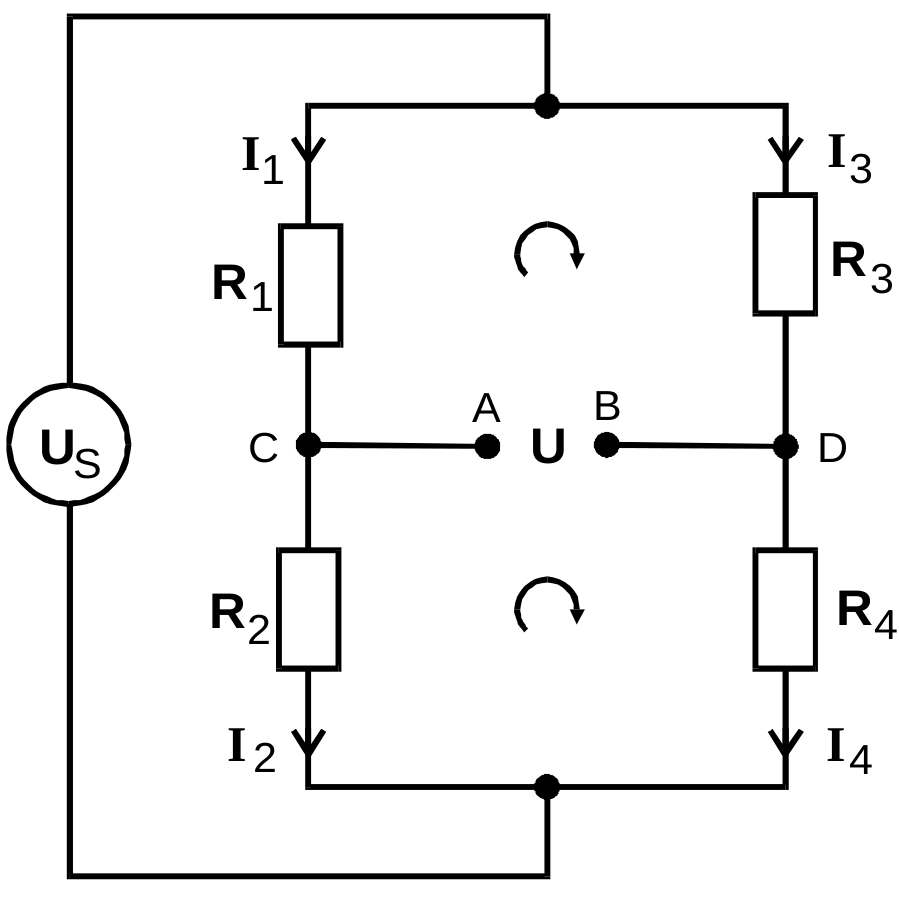
\includegraphics[width=0.5\textwidth]{Bilder/Brueckenschaltung.png}
  \caption{}
  \label{fig:}
\end{figure}
Die Wheatstonesche Brückenschaltung kann mit Wechsel und Gleichstrom betrieben werden,
da sie nur ohmsche Widerstände enthält. Die bekannten Widerstände $R_3$ $R_2$und $R_4$
 müssen so variiert werden, dass die Potentialdifferenz verschwindet. Mit der
Gleichung\eqref{eq:Widerstand} erhält man so den unbekannten Widerstand $R_x$
aus\eqref{eq:Widerstand_Rx}.
\begin{equation}
R_x=R_2 \frac{R_3}{R_4}
\label{eq:Widerstand_Rx1}
\end{equation}
Werden die Widerstände $R_1$ und $R_2$ durch zwei Kapazitäten der Form
\begin{equation}
\hat{Z}_{C_{real}}=R-\frac{i}{\omega C}  ,
\end{equation}
ersetzt, ergibt sich eine Kapazitätsmessbrücke  wie in Abbildung\ref{fig:capbruecke}.
Mit den Formeln \eqref{eq:Widerstand_Rx2} und \eqref{eq:Kapazitaet_Rx2}ergeben
sich die unbekannten Widerstände und Capazitäten.
\begin{equation}
R_x=R_2\frac{R_3}{R_4}
\label{eq:Widerstand_Rx2}
\end{equation}
\begin{equation}
C_x=C_2\frac{R_4}{R_3}
\label{eq:Kapazitaet_Rx2}
\end{equation}
\begin{figure}
  \centering
  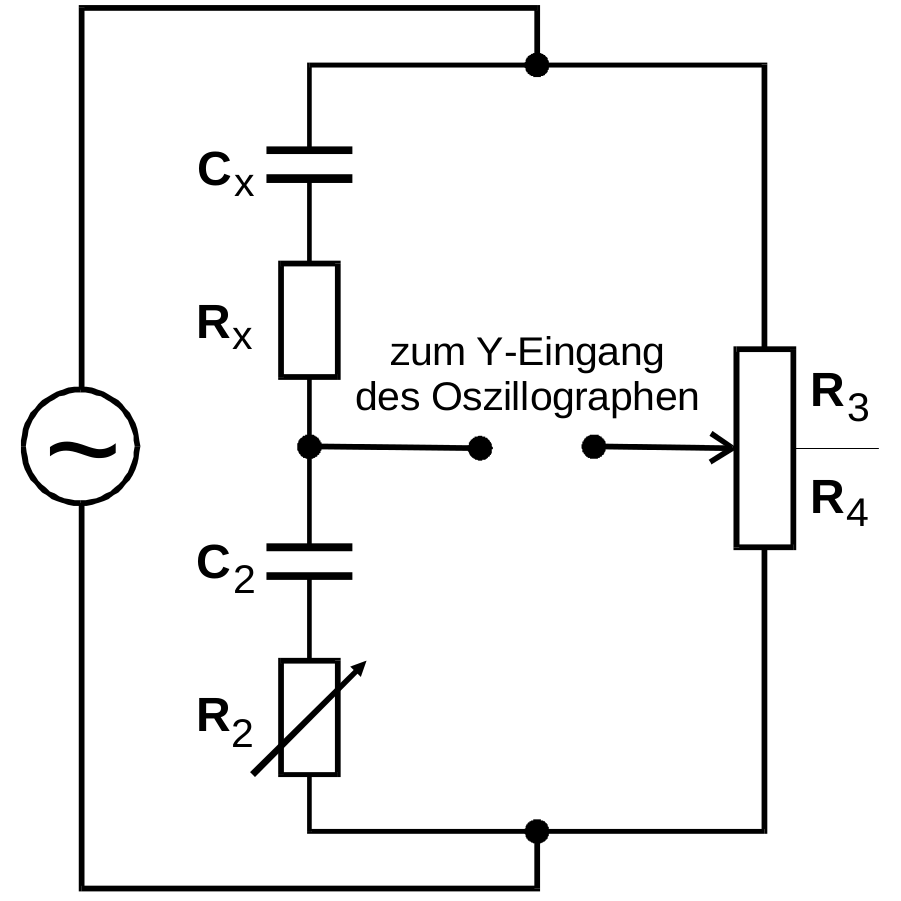
\includegraphics[width=0.5\textwidth]{Bilder/Capazitaetsbruecke.png}
  \caption{}
  \label{fig:capbruecke}
\end{figure}
Werden die Kapazitäten durch Induktivitäten ausgetauscht, ergibt sich eine
Induktivitätsmessbrücke wie in Abbildung\ref{fig:indbruecke}.
\begin{equation}
R_x=R_2\frac{R_3}{R_4}
\end{equation}
\begin{equation}
L_x=L_2 \frac{R_3}{R_4}
\end{equation}
\begin{figure}
  \centering
  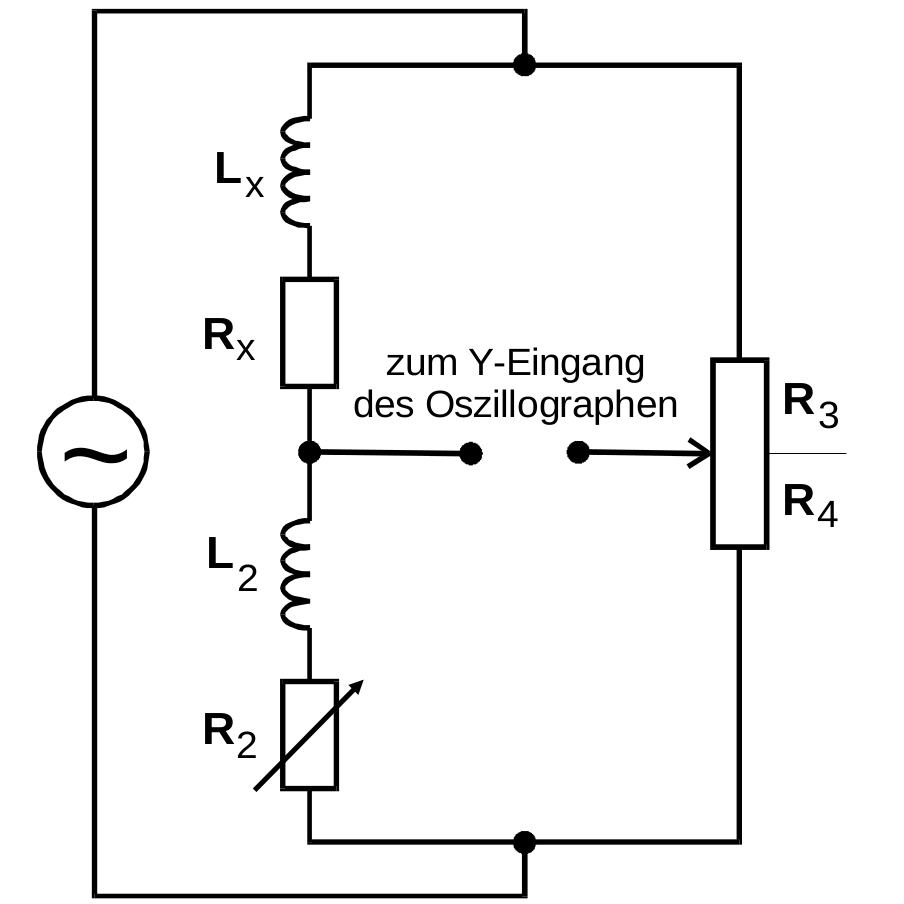
\includegraphics[width=0.5\textwidth]{Bilder/Induktivitaetsbruecke.png}
  \caption{}
  \label{fig:indbruecke}
\end{figure}
Mit einer Maxwellbrücke wie in Abbildung\ref{Bilder/Maxwell.png} lassen sich mit
den Gleichungen\eqref{eq:Widerstand3}\eqref{eq:Induktivitaet} unbekannte
Induktivitäten und Widerstände bestimmen.
\begin{equation}
R_x= \frac{R_2 R_3}{R_4}
\label{eq:Widerstand3}
\end{equation}
\begin{equation}
L_x=R_2 R_3 C_4
\label{eq:Induktivitaet}
\end{equation}
\begin{figure}
  \centering
  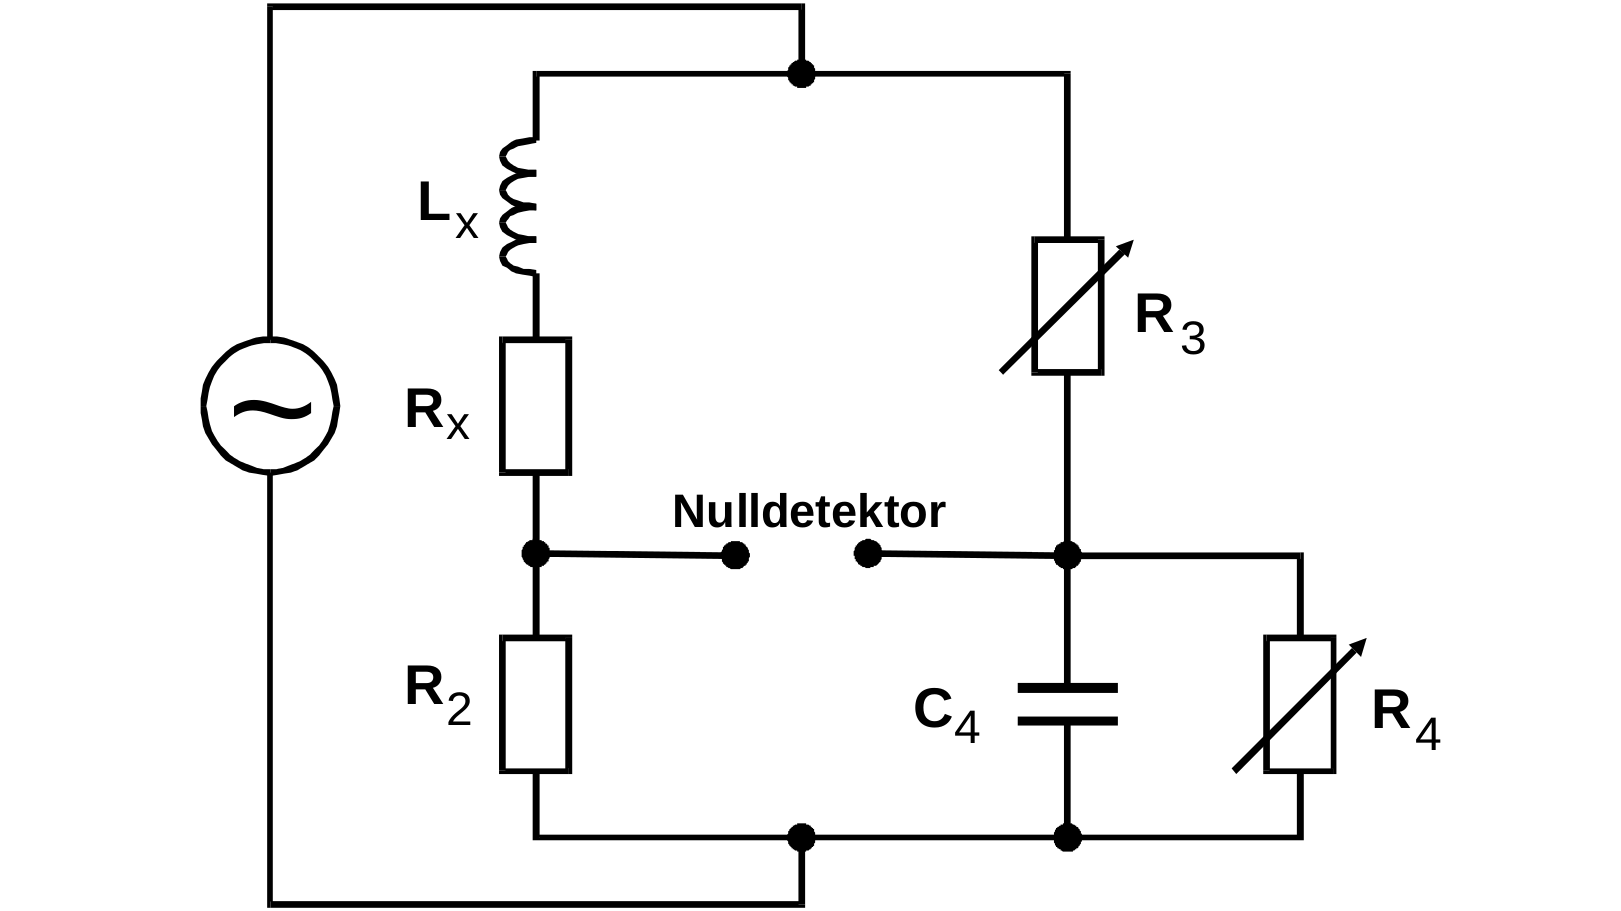
\includegraphics[width=0.5\textwidth]{Bilder/Maxwellbruecke.png}
  \caption{}
  \label{fig:Maxwellb}
\end{figure}
Mit einer Wien-Robinson-Brücke lässt sich eine genaue Messung nur bei einer
bestimmten Frequenz durchführen. Mit dieser lassen sich bestimmte Frequenzen der
Form
\begin{equation}
\omega_0=\frac{1}{RC}
\end{equation}
herausfilter, da die Brückenspannung dann $0$ ist.
\begin{figure}
  \centering
  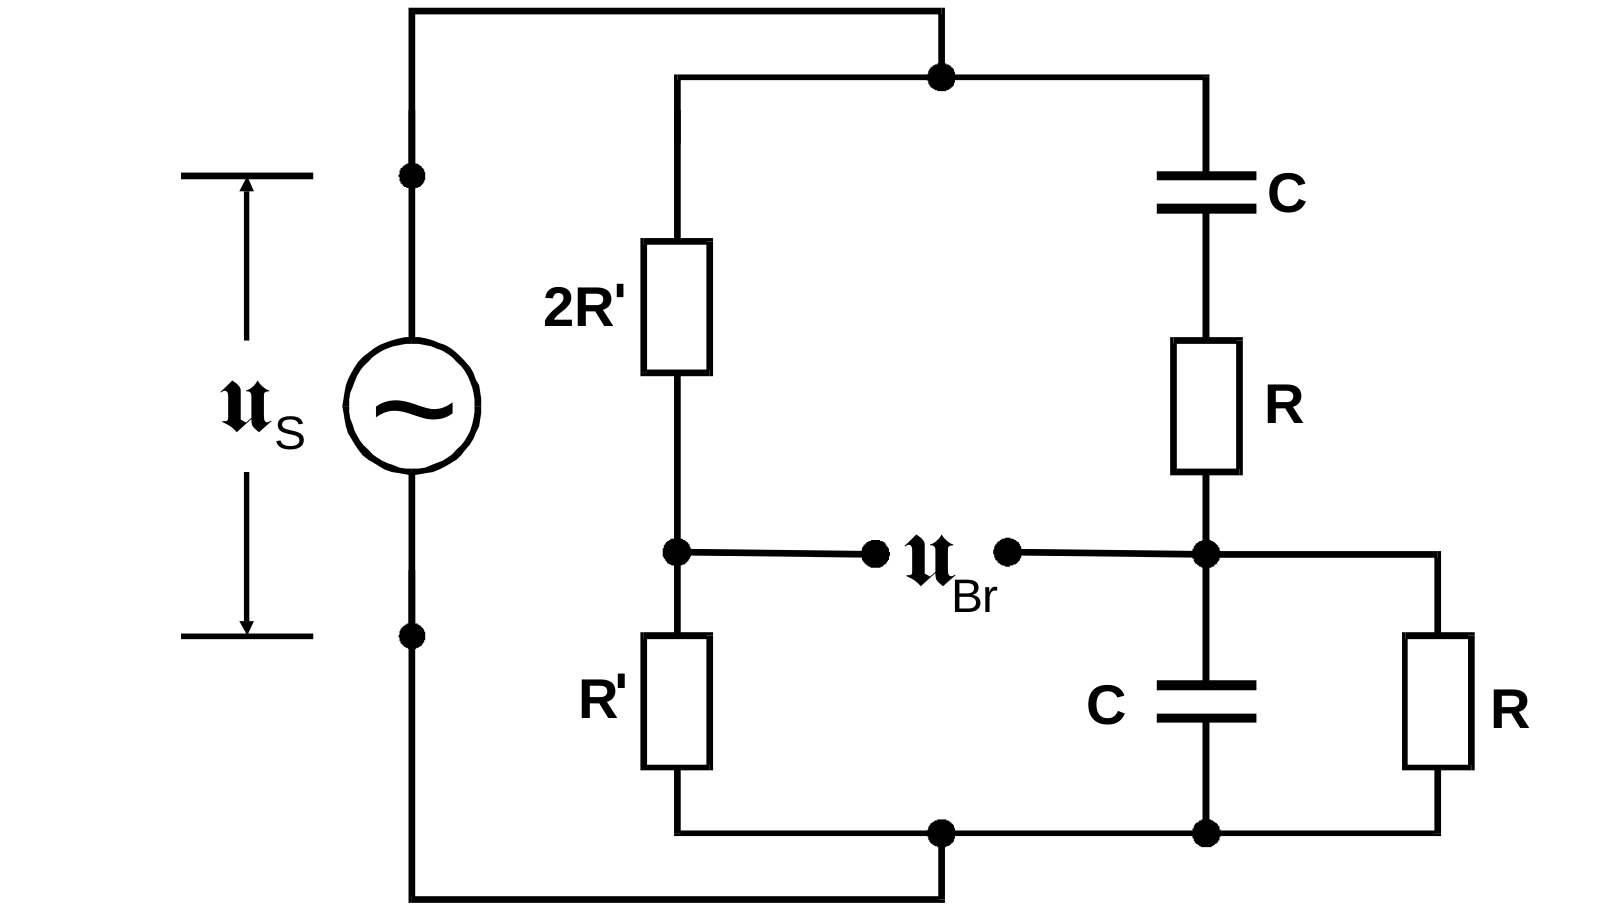
\includegraphics[width=0.5\textwidth]{Bilder/Wien_Robinsonbruecke.png}
  \caption{}
  \label{fig:Maxwellb}
\end{figure}
\begin{equation}
\frac{U_S}{U_{Br}}=\frac{1}{\omega}^2R^2C^2-1\left\{\,3(1-\omega^2 R^2 C^2)
+9i\omega RC \right\}
\end{equation}
\begin{equation}
\left|\frac{U_{Br}}{U_S}\right|^2=\frac{(\omega^2R^2C^2-1)^2}
{9\left\{(1-\omega^2 R^2 C^2)^2+9\omega^2R^2C^2\right\}}
\end{equation}
\begin{equation}
\Omega:=\frac{\omega}{\omega_0}
\end{equation}
\begin{equation}
\left|\frac{U_{Br}}{U_S}\right|^2=\frac{1}{9}\frac{(\Omega^2-1)^2}
{(1-\Omega^2)^2+9\Omega^2}
\end{equation}
